\begin{figure}[!h]
  \begin{center}
    \caption{Configurations possibles sous l'hypothèse qu'un point est visible}%
    \label{vis:ill}
    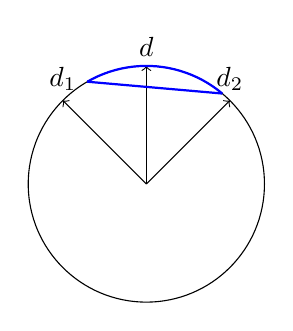
\begin{tikzpicture}[scale=1.5]
      \draw [thin] (0, 0) circle (1cm);
      \draw [->](0, 0) -- (90:1) node[above] {$d$};
      \draw [->] (0, 0) -- (45:1) node[above] {$d_2$};
      \draw [->] (0, 0) -- (135:1) node[above] {$d_1$};
      \draw [blue, thick, domain=50:120] plot ({cos(\x)}, {sin(\x)});
      \draw [thick, blue] (120:1) -- (50:1);
    \end{tikzpicture}
    % \begin{tikzpicture}[scale=1.5]
    %   \draw [thin] (0, 0) circle (1cm);
    %   \draw [->](0, 0) -- (90:1) node[above] {$d$};
    %   \draw [->] (0, 0) -- (45:1) node[above] {$d_2$};
    %   \draw [->] (0, 0) -- (135:1) node[above] {$d_1$};
    %   \draw [blue, thick, domain=-15:70] plot ({cos(\x)}, {sin(\x)});
    %   \draw [thick, blue] (-15:1) -- (70:1);
    % \end{tikzpicture}
    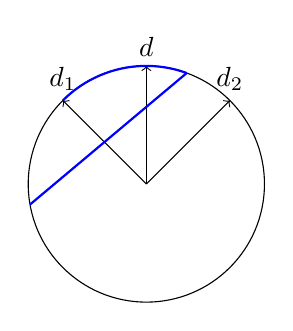
\begin{tikzpicture}[scale=1.5]
      \draw [thin] (0, 0) circle (1cm);
      \draw [->](0, 0) -- (90:1) node[above] {$d$};
      \draw [->] (0, 0) -- (45:1) node[above] {$d_2$};
      \draw [->] (0, 0) -- (135:1) node[above] {$d_1$};
      \draw [blue, thick, domain=70:135] plot ({cos(\x)}, {sin(\x)});
      \draw [thick, blue] (190:1) -- (70:1);
    \end{tikzpicture}
    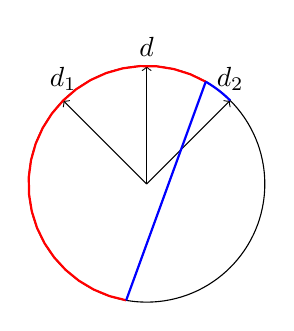
\begin{tikzpicture}[scale=1.5]
      \draw [thin] (0, 0) circle (1cm);
      \draw [->](0, 0) -- (90:1) node[above] {$d$};
      \draw [->] (0, 0) -- (45:1) node[above] {$d_2$};
      \draw [->] (0, 0) -- (135:1) node[above] {$d_1$};
      \draw [red, thick, domain=60:260] plot ({cos(\x)}, {sin(\x)});
      \draw [thick, blue] (260:1) -- (60:1);
      \draw [blue, thick, domain=45:60] plot ({cos(\x)}, {sin(\x)});
    \end{tikzpicture}
\end{center}
\end{figure}
%%% Local Variables:
%%% mode: latex
%%% TeX-master: "../rapportGp1"
%%% End:
